% =============================================================================
% Kapitel 3 -- Architektur & Design Patterns
% =============================================================================
\section{Architektur}

\subsection{Der GameManager als zentraler Koordinator}

Der \texttt{GameManager} ist das Herzstück von CardSiege. Er hält Referenzen auf
alle wesentlichen Spielobjekte: Spielfeld, Türme, Gegner, Projektile,
Kartensystem, aktuelle Phase, Ressourcen und den Ereignisbus und orchestriert
deren Zusammenspiel. Seine zentrale \texttt{update()}-Methode wird einmal pro
Frame vom \texttt{GameScreen} aufgerufen und koordiniert Gegnerbewegung,
Reichweitenüberwachung, Kampflogik und das Aufräumen besiegter Einheiten.
Sämtliche inhaltliche Verantwortung delegiert er dabei an spezialisierte
Teilsysteme, deren konkrete Umsetzung er nicht kennt. Wie diese Delegation
architektonisch strukturiert ist, beschreiben die folgenden Abschnitte.

% =============================================================================
\subsection{Singleton - GameManager}
% =============================================================================

Ein Tower-Defense-Spiel besitzt zu jedem Zeitpunkt genau einen definierten
Spielzustand. Turmlisten, Phasenzustand, Ressourcenzähler und der aktive
Ereignisbus müssen konsistent von einer einzigen Stelle verwaltet werden.
Würden mehrere \texttt{GameManager}-Instanzen existieren, könnten Türme in einer
Instanz registriert, Gegner aber in einer anderen verwaltet werden, das Spiel
wäre nicht mehr deterministisch steuerbar.

Der \texttt{GameManager} wird deshalb als Singleton mit \textit{Eager
Initialization} umgesetzt: Die einzige Instanz entsteht als statische
Klassenvariable beim Klassenladen der JVM, noch bevor irgendein Aufruf von
\texttt{get()} möglich ist. Ein privater Konstruktor verhindert externe
Instanziierung vollständig. Diese Variante wurde der lazy Alternative
(\texttt{if (INSTANCE == null)}) vorgezogen, weil das Spiel single-threaded
läuft und eine aufwändige Synchronisierung unnötig wäre.

\begin{lstlisting}[caption={Singleton mit Eager Initialization},label=lst:singleton]
public class GameManager {
    private static final GameManager INSTANCE = new GameManager();

    public static GameManager get() { return INSTANCE; }

    private GameManager() {
        eventBus.subscribe(new GameEventLogger()); // Observer sofort aktiv
    }
}
\end{lstlisting}

Bemerkenswert ist, dass der Konstruktor unmittelbar das Observer-System
initialisiert: Der \texttt{GameEventLogger} wird bereits im privaten Konstruktor
am \texttt{GameEventBus} registriert, sodass das Logging-System von der ersten
Spielaktion an aktiv ist, ohne explizite Initialisierungsreihenfolge nach außen.
Der bekannte Nachteil erschwerter Unit-Tests durch persistierenden globalen Zustand
wurde zugunsten der Einfachheit akzeptiert. In einem produktiven Kontext würde man
den \texttt{GameManager} per Dependency Injection übergeben.

% =============================================================================
\subsection{Factory Method - CardFactory}
% =============================================================================

Das Deck soll Karten erzeugen, ohne konkrete Kartentypen zu kennen. Wäre die
Erzeugungslogik direkt in der \texttt{Deck}-Klasse implementiert, würde jede
neue Karte eine Änderung im Deck-Code erzwingen, eine direkte Verletzung des
Open/Closed Principle. Das Problem liegt darin, dass Erzeugung und Verwaltung
von Karten zwei grundlegend verschiedene Verantwortlichkeiten sind, die
voneinander getrennt gehören.

Das Interface \texttt{CardFactory} definiert eine einzige Methode
\texttt{createDeck()}, die eine Liste fertig konfigurierter Karten zurückgibt.
Das \texttt{Deck} kennt ausschließlich dieses Interface, nie eine konkrete
Kartenklasse. Die gesamte Entscheidung darüber, welche Karten mit welchen
Parametern im Deck landen, liegt in der konkreten Implementierung
\texttt{StrategyCardFactory}. Diese bestückt das Deck mit zehn Kartentypen: drei
Turmkarten (Scout, Sniper, Rapid) mit ihren jeweiligen Strategie-Kombinationen
sowie sieben Karten für Ressourcen, Buffs und Sondereffekte. Ein alternativer
Kartensatz für einen anderen Schwierigkeitsgrad oder ein Tutorial ließe sich
vollständig durch eine neue \texttt{CardFactory}-Implementierung einführen, ohne
eine einzige Zeile in \texttt{Deck} zu ändern.

\begin{lstlisting}[caption={Factory-Interface und Nutzung im Deck},label=lst:factory]
public interface CardFactory {
    List<Card> createDeck();
}

// Deck kennt nur das Interface, nie konkrete Kartenklassen:
private void refill() {
    for (Card proto : factory.createDeck()) {
        cards.add(proto.copy()); // Prototype Pattern
        cards.add(proto.copy());
    }
    Collections.shuffle(cards);
}
\end{lstlisting}

Das unmittelbare Zusammenspiel mit dem Prototype-Pattern ist an dieser Stelle
besonders deutlich: Die Factory liefert konfigurierte Prototypen, das Deck klont
jeden zweimal, um zwanzig Karten zu erhalten. Weder Deck noch Factory wissen
voneinander, wie die Objekte intern konstruiert sind.

% =============================================================================
\subsection{Prototype - Card.copy() und EnemyPrototype}
% =============================================================================

Das Prototype-Pattern adressiert in CardSiege dasselbe konzeptionelle Problem an
zwei verschiedenen Stellen: Konfigurierte Objekte sollen geklont werden, anstatt
ihre Parameter bei jeder Erzeugung erneut angeben zu müssen. Ohne Prototype
müsste die Konfiguration, etwa Geschwindigkeit und Trefferpunkte eines
Gegnertyps, an jeder Spawn-Stelle im Code wiederholt werden, was zu
Inkonsistenzen führen und Änderungen aufwändig machen würde.

Im Kartensystem schreibt die abstrakte Basisklasse \texttt{Card} die Methode
\texttt{copy()} vor, die jede konkrete Kartenklasse implementiert. Das Deck ruft
\texttt{copy()} beim Befüllen auf und erhält so frische Instanzen mit identischem
Zustand, die aber voneinander unabhängig sind, das Ausspielen einer Karte
beeinflusst keinen anderen Kartenstapel. Die Klon-Logik im Deck bleibt dabei
stabil, egal wie viele neue Kartentypen hinzukommen.

Im Gegnersystem hält der \texttt{WaveSpawner} drei konfigurierte
\texttt{EnemyPrototype}-Objekte, einen für jeden Gegnertyp. Die Attribute werden
einmal pro Welle festgelegt und skalieren mit der Wellennummer. Bei jedem
Spawn-Vorgang wird der passende Prototyp über \texttt{copy(path)} geklont,
wobei der aktuelle Spielfeldpfad mitgegeben wird, da jeder Gegner seinen eigenen,
unabhängigen Fortschritt auf dem Pfad verfolgt.

\begin{lstlisting}[caption={Prototype im WaveSpawner},label=lst:prototype]
// Einmalig pro Welle konfiguriert:
standardEnemy = new EnemyPrototype(EnemyType.STANDARD, baseSpeed, baseHp);

// Pro Spawn geklont, Konfiguration zentral, Pfadfortschritt immer frisch:
manager.spawnEnemy(selectPrototype(index).copy(manager.getBoard().getPath()));
\end{lstlisting}

Dass dasselbe Pattern an zwei unabhängigen Stellen eingesetzt wird, illustriert
seine Vielseitigkeit. In beiden Fällen liegt der Kern des Problems nicht in der
Erzeugung an sich, sondern in der zentralen Verwaltung von Konfiguration: Es
soll eine einzige, verlässliche Quelle der Wahrheit für die Eigenschaften eines
Objekttyps geben.

% =============================================================================
\subsection{Builder - PendingTower}
% =============================================================================

Wenn der Spieler eine Turmkarte ausspielt, ist zu diesem Zeitpunkt ein
wesentlicher Parameter noch unbekannt: die Gitterkoordinaten, auf denen der
Turm platziert werden soll. Der Spieler muss erst auf ein gültiges Spielfeld-Feld
klicken. Eine direkte Erzeugung des Turms beim Kartenspielen ist damit nicht
möglich, der Bauprozess ist zwingend zweistufig.

Das Builder-Pattern trennt deshalb die Konfiguration des Turms von seiner
Instanziierung. Wenn eine \texttt{BuildTowerCard} ausgespielt wird, erzeugt sie
einen \texttt{PendingTower}, der alle bereits bekannten Parameter speichert:
Name, Typ, Kosten, Basisschaden, Reichweite, Cooldown sowie die gewählten
Targeting- und Angriffsstrategien. Ein \texttt{BaseTower} wird zu diesem
Zeitpunkt noch nicht erzeugt. Erst wenn der Spieler auf ein gültiges Feld
klickt, ruft der Manager \texttt{PendingTower.build(gridX, gridY)} auf und
übergibt die nun bekannten Koordinaten.

\begin{lstlisting}[caption={Zweistufige Turmerzeugung mit PendingTower},label=lst:builder]
// Schritt 1 - Karte ausgespielt, Koordinaten noch unbekannt:
context.getManager().queueTowerPlacement(new PendingTower(...));

// Schritt 2 - Spieler klickt Zielfeld, Koordinaten jetzt bekannt:
public TowerComponent build(int gridX, int gridY) {
    return new BaseTower(name, type, gridX, gridY, baseDamage,
                         range, cooldown, cost, targeting, attackStrategy);
}
\end{lstlisting}

Diese Trennung hat einen praktischen Nebennutzen, der direkt aus der
Architekturentscheidung erwächst: Solange ein \texttt{PendingTower} aktiv ist,
rendert der \texttt{GameScreen} einen Platzierungsmarker mit Reichweitenkreis
auf dem Spielfeld. Der Spieler sieht visuell, welchen Bereich der Turm abdecken
würde, bevor er die endgültige Entscheidung trifft, ohne dass dafür ein echter
Turm existieren müsste. Das Builder-Pattern liefert hier also nicht nur
sauberere Objekterzeugung, sondern ermöglicht direkt ein UI-Feature.

% =============================================================================
\subsection{Decorator - Turmerweiterungssystem}
% =============================================================================

Das Decorator-Pattern ist die architektonisch prägendste Entscheidung im Projekt,
weil sie ihren Nutzen im direkten Vergleich zur Alternative am deutlichsten
demonstriert. Türme sollen zur Laufzeit mit Boni ausgestattet werden können:
Eine Buff-Karte erhöht den Schaden aller Türme, eine andere erhöht die Reichweite
eines einzelnen Turms, ein Upgrade verbessert Level, Schaden und Cooldown
gleichzeitig. Diese Boni können in beliebiger Reihenfolge und Kombination
auf einen Turm angewendet werden.

Die naheliegende Alternative wäre Vererbung: Für jede mögliche Kombination aus
Turmtyp und Buffzustand eine eigene Klasse. Mit drei Turmtypen und drei Bufftypen
wären das bereits 24 Klassen, die bei jedem neuen Bufftyp weiter explodieren.
Das Decorator-Pattern löst dieses Problem fundamental anders: Alle Türme und alle
Dekoratoren implementieren dasselbe Interface \texttt{TowerComponent}. Die
abstrakte Klasse \texttt{TowerDecorator} hält eine Referenz auf ein inneres
\texttt{TowerComponent} und delegiert alle Methoden per Default daran. Konkrete
Dekoratoren überschreiben ausschließlich die Methoden, für die sie einen Bonus
liefern.

\begin{lstlisting}[caption={Delegation und gezielte Überschreibung im Decorator},label=lst:decorator]
public abstract class TowerDecorator implements TowerComponent {
    protected final TowerComponent inner;
    @Override public int getDamage()     { return inner.getDamage(); }
    @Override public float getRange()    { return inner.getRange(); }
    // alle anderen Methoden delegieren analog ...
}

public class DamageBuffDecorator extends TowerDecorator {
    private final int bonusDamage;
    @Override
    public int getDamage() { return inner.getDamage() + bonusDamage; }
}
\end{lstlisting}

\begin{figure}[H]
    \centering
    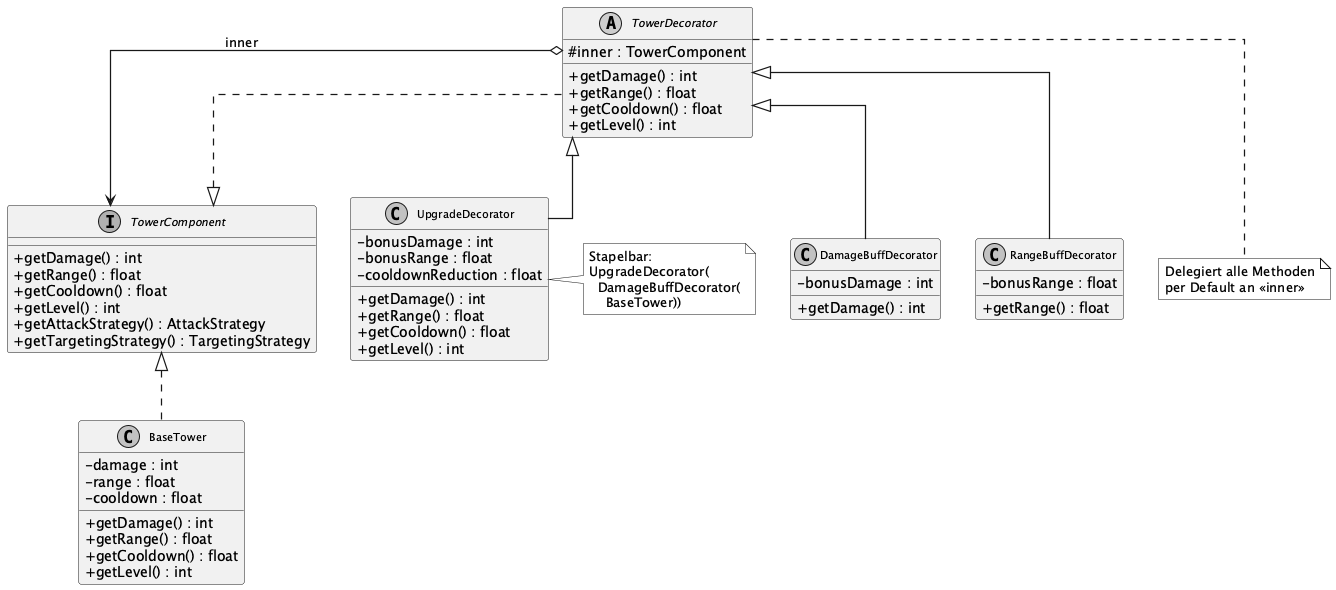
\includegraphics[width=\textwidth]{diagrams/decorator}
    \caption{Decorator-Pattern: \texttt{TowerComponent}-Hierarchie mit stapelbaren Dekoratoren}
    \label{fig:decorator}
\end{figure}

Dekoratoren lassen sich beliebig stapeln. Ein Aufruf von \texttt{getDamage()}
auf einem \texttt{UpgradeDecorator(DamageBuffDecorator(BaseTower))} traversiert
transparent die gesamte Kette und summiert alle Boni auf. Die restliche
Spiellogik, Strategy und GameManager, sieht stets nur ein
\texttt{TowerComponent} und muss nichts von der Decorator-Kette wissen.
Neue Bufftypen lassen sich vollständig ohne Änderung bestehender Klassen
ergänzen.

% =============================================================================
\subsection{Command - Kartensystem}
% =============================================================================

Das Command-Pattern kapselt jede Spielaktion als eigenständiges Objekt. Die
abstrakte Basisklasse \texttt{Card} definiert das Command-Interface mit der
Methode \texttt{execute(CardContext)}. Jede konkrete Kartenklasse ist ein
ConcreteCommand: Sie kennt ausschließlich ihren eigenen Parameter, etwa den
Schadenswert oder die Langsamdauer, und delegiert die Ausführung vollständig
an den Receiver.

Der \texttt{GameManager} übernimmt die Receiver-Rolle. Er stellt für jede
Spielaktion eine semantisch benannte Methode bereit:
\texttt{applyDamageBuff()}, \texttt{queueRangeBuff()} und
\texttt{slowAllEnemies()} kapseln die jeweilige Implementierungslogik, etwa
die Konstruktion von Decorator-Objekten oder die Iteration über die
Gegnerliste. Die Karten wissen \textit{was} ausgelöst werden soll, der
\texttt{GameManager} weiß \textit{wie} es intern umgesetzt wird.

\begin{lstlisting}[caption={Command-Pattern: DamageBuffCard delegiert an den Receiver},label=lst:command]
// ConcreteCommand kennt nur seinen Parameter
public void execute(CardContext context) {
    context.getManager().applyDamageBuff(bonusDamage);
}

// Receiver kennt die Implementierungsdetails
public void applyDamageBuff(int bonusDamage) {
    applyTowerModifier(tower -> new DamageBuffDecorator(tower, bonusDamage));
}
\end{lstlisting}

Der \texttt{GameScreen} agiert als Invoker: Er ruft \texttt{playCard(index)}
auf dem \texttt{GameManager} auf, ohne konkrete Kartentypen zu kennen.
Die acht Kartenklassen, \texttt{DamageBuffCard}, \texttt{RangeBuffCard},
\texttt{FreezeCard}, \texttt{EnergyCard}, \texttt{GoldCard}, \texttt{DrawCard},
\texttt{DiscountCard} und \texttt{BuildTowerCard}, sind alle nach demselben
Prinzip aufgebaut: ein schlankes Aktionsobjekt, ein Receiver-Aufruf.

Das Command-Pattern kooperiert eng mit dem Decorator-Pattern:
\texttt{applyDamageBuff()} und \texttt{queueRangeBuff()} sind die einzigen
Stellen im System, an denen Decorator-Objekte erzeugt werden. Die Karten
kennen \textit{dass} ein Buff stattfindet, nicht \textit{wie} er durch
gestapelte Wrapper realisiert wird. Eine \texttt{undo()}-Methode auf dem
Command-Interface ist nicht implementiert, da Decorator-Ketten nicht trivial
rückgängig gemacht werden können.

% =============================================================================
\subsection{Strategy - Zielwahl und Angriffsverhalten}
% =============================================================================

Turmtypen unterscheiden sich in zwei voneinander unabhängigen Dimensionen:
\textit{wen} sie angreifen (Zielwahl) und \textit{wie} sie angreifen
(Angriffstyp). Scout und Sniper verwenden Einzelschuss, Rapid verteilt
Flächenschaden. Scout priorisiert den Gegner mit dem größten Fortschritt auf dem
Pfad, Sniper den mit den meisten Lebenspunkten. Diese Dimensionen sind
orthogonal, jede Kombination ist denkbar und sinnvoll einsetzbar.

Würde man diese Unterschiede direkt in den Turmklassen codieren, etwa durch
eine \texttt{switch}-Anweisung über den Turmtyp, müsste bei jedem neuen Turmtyp
oder jeder neuen Angriffsvariante die Turmklasse geändert werden. Das verletzt
das Single-Responsibility Principle und führt zu wachsenden, schwer lesbaren
Klassen.

Das Strategy-Pattern trennt die beiden Dimensionen in zwei Interfaces:
\texttt{TargetingStrategy} kapselt die Zielwahl, \texttt{AttackStrategy} die
Angriffsausführung. Jeder Turm erhält bei seiner Erzeugung durch die
\texttt{StrategyCardFactory} eine konkrete Kombination beider Strategien und
delegiert beim Feuern vollständig an sie. Die vier möglichen Kombinationen
aus zwei Targeting- und zwei Angriffsstrategien entstehen ohne eine einzige
zusätzliche Klasse.

\begin{figure}[H]
    \centering
    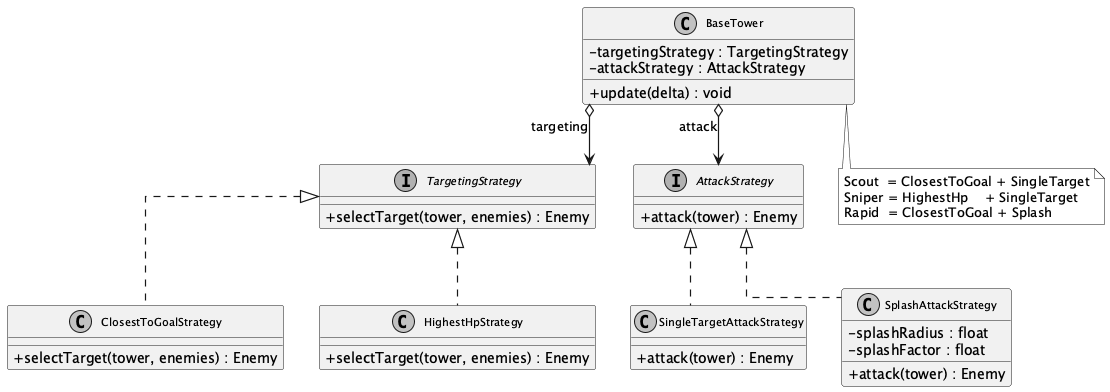
\includegraphics[width=\textwidth]{diagrams/strategy}
    \caption{Strategy-Pattern: zwei orthogonale Verhaltens-Dimensionen, zusammengeführt im \texttt{BaseTower}}
    \label{fig:strategy}
\end{figure}

Das Zusammenspiel mit dem Decorator-Pattern ist besonders subtil: Wenn die
\texttt{SplashAttackStrategy} \texttt{tower.getDamage()} aufruft, traversiert
dieser Aufruf transparent eine möglicherweise mehrschichtige Decorator-Kette.
Die Strategie erhält stets den kumulierten, gebufften Schadenswert, ohne davon
zu wissen. Die Entkopplung funktioniert vollständig über das gemeinsame Interface
\texttt{TowerComponent}.

% =============================================================================
\subsection{State - Spielphasenzyklus}
% =============================================================================

Der Spielablauf gliedert sich in einen geschlossenen Viererzyklus:
\textit{Draw} $\rightarrow$ \textit{Play} $\rightarrow$ \textit{Wave}
$\rightarrow$ \textit{Resolve} $\rightarrow$ \textit{Draw} $\rightarrow$ \ldots\
Jede Phase bringt eigene Regeln mit: In der Draw-Phase werden Karten gezogen und
Energie aufgefüllt, in der Play-Phase spielt der Spieler Karten aus und
positioniert Türme, in der Wave-Phase läuft die Gegnerwelle während Buff-Karten
weiterhin einsetzbar sind, und die Resolve-Phase leitet nach kurzem Delay den
nächsten Zug ein. Zwölf abgeschlossene Wellen führen zum Sieg, fehlende
Basislebenspunkte zur Niederlage.

Ohne das State-Pattern würde der \texttt{GameManager} ein wachsendes Geflecht
aus phasenabhängigen Bedingungen verwalten: Karten dürfen nur in bestimmten
Phasen ausgespielt werden, Gegner spawnen nur in der Wave-Phase, der nächste Zug
beginnt erst nach Ablauf eines Timers. All dieses Verhalten in einer einzigen
Klasse zu konzentrieren würde zu unübersichtlichen
\texttt{if~(currentPhase~==~...)}-Ketten führen, die mit jeder neuen Phase
schwerer wartbar werden.

Das State-Pattern kapselt das Verhalten jeder Phase vollständig in einer eigenen
Klasse, die das Interface \texttt{GamePhase} implementiert. Dieses schreibt drei
Methoden vor: \texttt{getName()} liefert den Phasennamen, \texttt{enter()} wird
einmalig beim Betreten der Phase aufgerufen und enthält Initialisierungslogik,
\texttt{update()} wird in jedem Frame aufgerufen und enthält das laufende
Verhalten. Der \texttt{GameManager} kennt keine Phasenlogik, er ruft lediglich
\texttt{phase.update()} auf und wechselt die Phase auf Anforderung.

\begin{lstlisting}[caption={Phasenwechsel im GameManager und Beispielphase},label=lst:state]
// GameManager delegiert vollstaendig an die aktive Phase:
public void switchPhase(GamePhase newPhase) {
    this.phase = newPhase;
    newPhase.enter(this);
    eventBus.publish(GameEvent.phaseChanged(newPhase.getName()));
}

// DrawPhase initialisiert den Zug und wechselt sofort weiter:
public void enter(GameManager manager) {
    manager.drawHand(3);
    manager.resetEnergy(3);
    manager.switchPhase(new PlayPhase());
}
\end{lstlisting}

\begin{figure}[H]
    \centering
    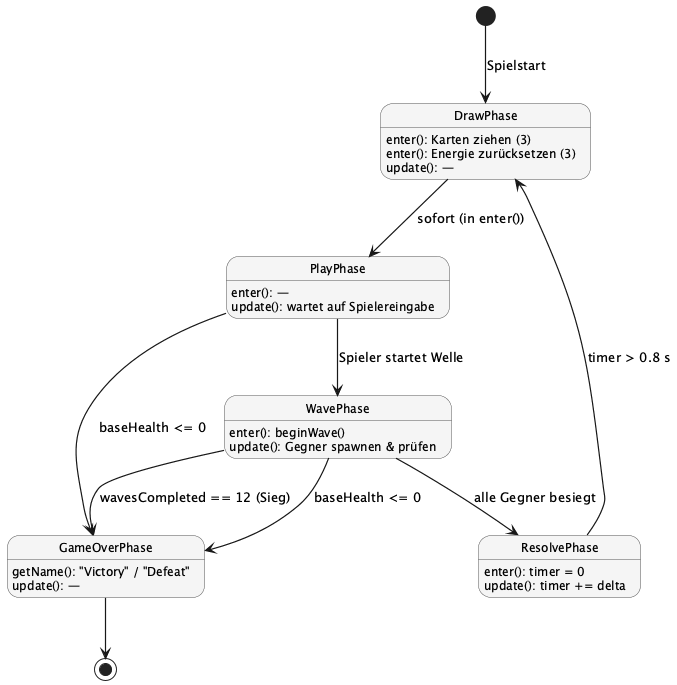
\includegraphics[width=0.82\textwidth]{diagrams/state}
    \caption{State-Pattern: Zustandsübergänge im Spielphasenzyklus}
    \label{fig:state}
\end{figure}

Die fünf Phasenklassen zeigen, wie sauber das Verhalten lokalisiert ist. Die
\texttt{DrawPhase} hat eine leere \texttt{update()}-Methode, weil sie ihre
gesamte Logik in \texttt{enter()} abarbeitet und sofort weiterleitet. Die
\texttt{PlayPhase} hat leere Implementierungen beider Methoden, weil sie
ausschließlich auf externe Nutzerinteraktion wartet, der Übergang in die
\texttt{WavePhase} wird vom \texttt{GameScreen} ausgelöst. Die
\texttt{ResolvePhase} verwaltet einen internen Timer und löst nach 0,8~Sekunden
selbstständig den nächsten Zug aus. Die \texttt{GameOverPhase} schließlich
bleibt in beiden Methoden leer: Das Spiel ist eingefroren, kein automatischer
Übergang findet statt. Dass jede Phase exakt die Methoden füllt, die sie
braucht, und alle anderen leer lässt, macht das phasenspezifische Verhalten
auf einen Blick sichtbar.

Das State-Pattern kooperiert unmittelbar mit dem Observer-Pattern: Jeder Aufruf
von \texttt{switchPhase()} publiziert automatisch ein \texttt{PhaseChanged}-Event
über den \texttt{GameEventBus}, ohne dass die aufrufende Phase davon wissen muss.

% =============================================================================
\subsection{Observer - GameEventBus}
% =============================================================================

Im Spielverlauf entstehen kontinuierlich bedeutsame Ereignisse: Ein Turm wird
gebaut, ein Gegner besiegt, eine Phase wechselt, die Basis erleidet Schaden.
Systeme wie ein Logger, ein Sound-Modul oder ein Statistik-Tracker sollen auf
diese Ereignisse reagieren, ohne dass der \texttt{GameManager} direkte
Abhängigkeiten zu ihnen aufbaut. Würde der Manager Logger oder UI direkt
referenzieren, entstünde enge Kopplung: Jede neue reaktive Komponente würde
Manager-Code erzwingen und die Klasse weiter aufblähen.

Das Observer-Pattern kehrt diese Abhängigkeit um. Der \texttt{GameEventBus}
verwaltet eine Liste von \texttt{GameEventListener}-Implementierungen und
benachrichtigt sie synchron bei jedem publizierten Ereignis. Die Abhängigkeit
zeigt nun in die entgegengesetzte Richtung: Nicht der Manager kennt den Logger,
sondern der Logger registriert sich selbst am Manager, zur Initialisierungszeit,
im privaten Singleton-Konstruktor.

Statt einfacher String-Konstanten verwendet das System typisierte Factory-Methoden
auf der \texttt{GameEvent}-Klasse: \texttt{GameEvent.towerBuilt(x,~y)},
\texttt{GameEvent.phaseChanged(name)} oder \texttt{GameEvent.baseDamaged(hp)}.
Diese Methoden konstruieren Events auf lesbare Weise und verhindern die Streuung
von Magic-Strings über die Codebasis. Gleichzeitig bleibt \texttt{GameEvent}
ein einfaches Wertobjekt ohne Vererbungshierarchie, der Ereignisname trägt
alle nötigen Informationen.

Aktuell ist der \texttt{GameEventLogger} der einzige Subscriber; er schreibt
jedes Ereignis auf die Konsole und macht den Spielverlauf nachvollziehbar. Die
Architektur ist dabei bereits für Erweiterungen offen: Ein Achievement-System,
ein Sound-Manager oder ein Replay-Recorder könnten sich mit einem einzigen
\texttt{eventBus.subscribe()}-Aufruf registrieren, ohne eine Zeile im
\texttt{GameManager} oder in bestehenden Listenern zu ändern. Das
Observer-Pattern liefert damit eine Infrastruktur, deren Erweiterbarkeit weit
über den aktuellen Nutzungsumfang hinausgeht.
